\hypertarget{a00001}{
\section{eqOsg::Application Class Reference}
\label{a00001}\index{eqOsg::Application@{eqOsg::Application}}
}
Sets up the whole \hyperlink{a00045}{eqOsg} Equalizer application.  


{\tt \#include $<$Application.h$>$}

Collaboration diagram for eqOsg::Application:\nopagebreak
\begin{figure}[H]
\begin{center}
\leavevmode
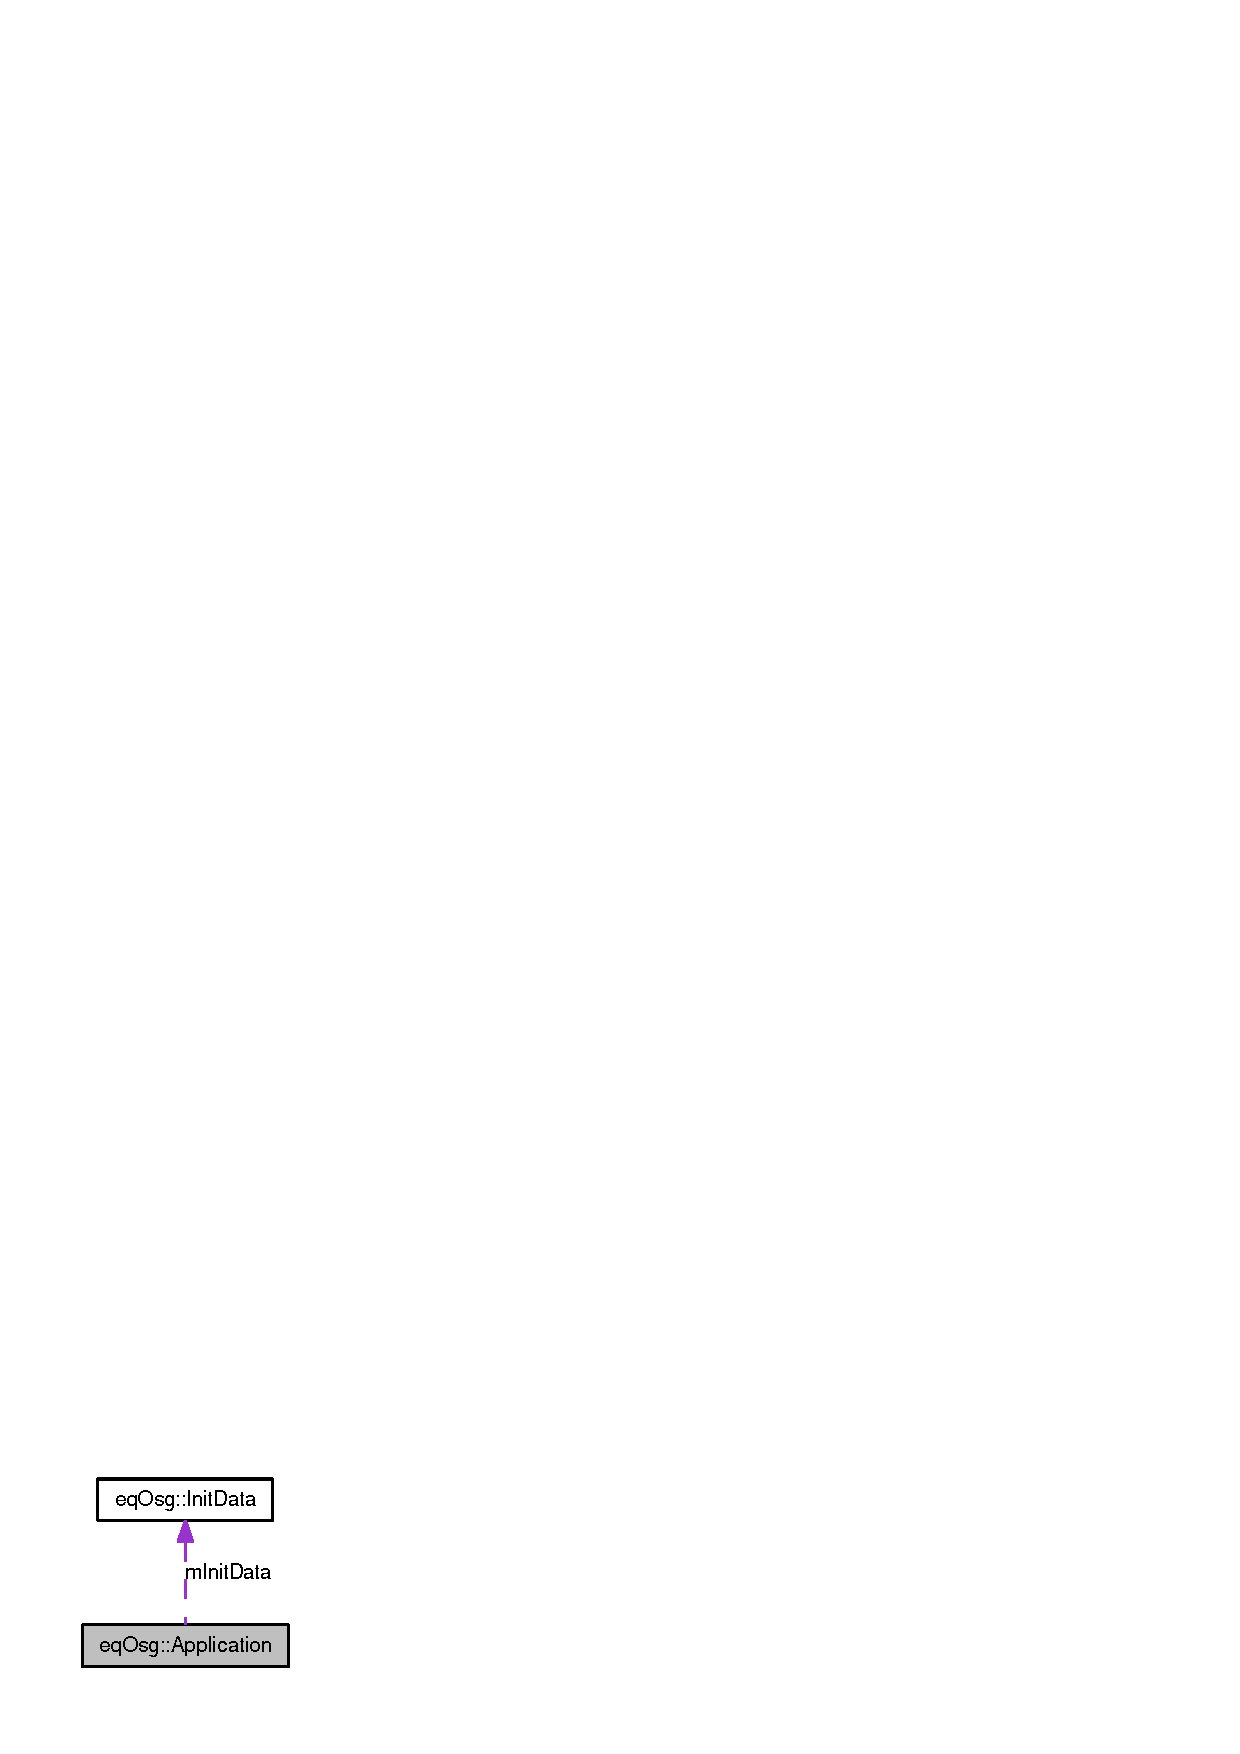
\includegraphics[width=142pt]{a00083}
\end{center}
\end{figure}
\subsection*{Public Member Functions}
\begin{CompactItemize}
\item 
\hyperlink{a00001_004ad4bb523a1a7ffe7a3e53c3eb82e2}{Application} (const \hyperlink{a00011}{InitData} \&initData)
\begin{CompactList}\small\item\em Constructor to pass the init data class. \item\end{CompactList}\item 
\hypertarget{a00001_8cf8941c8db90117d3735bce5ae1fdf4}{
int \hyperlink{a00001_8cf8941c8db90117d3735bce5ae1fdf4}{run} ()}
\label{a00001_8cf8941c8db90117d3735bce5ae1fdf4}

\begin{CompactList}\small\item\em Run this equalizer application. \item\end{CompactList}\end{CompactItemize}
\subsection*{Protected Member Functions}
\begin{CompactItemize}
\item 
\hypertarget{a00001_8b3cb53c57a36c01761b4fe74f9adbb0}{
virtual bool \hyperlink{a00001_8b3cb53c57a36c01761b4fe74f9adbb0}{clientLoop} ()}
\label{a00001_8b3cb53c57a36c01761b4fe74f9adbb0}

\begin{CompactList}\small\item\em The equalizer client loop. \item\end{CompactList}\end{CompactItemize}


\subsection{Detailed Description}
Sets up the whole \hyperlink{a00045}{eqOsg} Equalizer application. 

Contains the Equalizer main loop. 

\subsection{Constructor \& Destructor Documentation}
\hypertarget{a00001_004ad4bb523a1a7ffe7a3e53c3eb82e2}{
\index{eqOsg::Application@{eqOsg::Application}!Application@{Application}}
\index{Application@{Application}!eqOsg::Application@{eqOsg::Application}}
\subsubsection[{Application}]{\setlength{\rightskip}{0pt plus 5cm}Application::Application (const {\bf InitData} \& {\em initData})}}
\label{a00001_004ad4bb523a1a7ffe7a3e53c3eb82e2}


Constructor to pass the init data class. 

\begin{Desc}
\item[Parameters:]
\begin{description}
\item[{\em initData}]The destributet init data object \end{description}
\end{Desc}


The documentation for this class was generated from the following files:\begin{CompactItemize}
\item 
E:/schule/Thesis/Repo/trunk/crf/src/Application.h\item 
E:/schule/Thesis/Repo/trunk/crf/src/Application.cpp\end{CompactItemize}
